% !TeX encoding = UTF-8 Unicode
% !TeX root = main.tex
% !TeX TS-program = pdflatex
%% (При смене движка необходимо удалить вспомогательные файлы *.aux *.brf *.log *.out *.synctex.gz *.toc)

\documentclass{thesisby}
\usepackage{etoolbox,ifxetex,ifluatex}
\usepackage[unicode,hypertexnames=false]{hyperref}

%%% Проверка используемого TeX-движка %%%
\ifboolexpr{bool{xetex} or bool{luatex}}{%
  \usepackage{fontspec}
  \PassOptionsToPackage{no-math}{fontspec}     % https://tex.stackexchange.com/a/26295/104425
  \usepackage{polyglossia}%[2014/05/21]        % Поддержка многоязычности

  % fonts and languages
  \defaultfontfeatures{Ligatures=TeX,Mapping=tex-text}

  \setmainlanguage[babelshorthands = true]{russian}
  \setotherlanguage{english}

  \setmainfont{Times New Roman}
  \setmonofont{Courier New}
  \setsansfont{Arial}

  \newfontfamily\cyrillicfont[Script=Cyrillic]{Times New Roman}
  \newfontfamily\cyrillicfontsf[Script=Cyrillic]{Arial}
  \newfontfamily\cyrillicfonttt[Script=Cyrillic]{Courier New}

  \newfontfamily\englishfont{Times New Roman}
  \newfontfamily\englishfontsf{Arial}
  \newfontfamily\englishfonttt{Courier New}

  \renewcommand{\UrlFont}{\small\rmfamily\tt}
}{%
  \usepackage[T1,T2A]{fontenc}
  \usepackage[utf8]{inputenc}
  \usepackage[english, russian]{babel}
  \usepackage{csquotes}
  \IfFileExists{pscyr.sty}{\usepackage{pscyr}}{}  % Подключение pscyr
}

% Для борьбы с переполнениями за счет разреженных слов в абзаце
\emergencystretch=25pt

\usepackage{enumitem}

\usepackage[
    language = auto,        % Получение языка из babel.
    autolang = other,       % Многоязычная библиография.
    defernumbers = true,    % Раздельная нумерация.
    style = gost-numeric,
    maxnames = 10,
    movenames = false,
    sorting = ynt
]{biblatex} % To load multiple bib files.

% Библиографический список в соответствии с ГОСТ.
\makeatletter
\ltx@iffilelater{biblatex-gost.def}{2017/02/01}%
{\toggletrue{bbx:gostbibliography}%
    \renewcommand*{\revsdnamepunct}{\addcomma}}{}
\makeatother

% Общий список.
\addbibresource{references.bib}

% Список публикаций соискателя.
\addbibresource{references.bib}
\DeclareSourcemap{
    \maps[datatype=bibtex, overwrite]{
        \map{
            \perdatasource{references.bib}
            \step[fieldset=KEYWORDS, fieldvalue=ys, append]
        }
    }
}

% Счётчики.
\usepackage[figure,table]{totalcount}   % Счётчик рисунков и таблиц.
\usepackage{totcount}                   % Пакет создания счётчиков на основе последнего номера подсчитываемого элемента (может требовать дважды компилировать документ).
\AtEveryBibitem{\stepcounter{citenum}\stepcounter{citenum_my}}

\usepackage{totpages}
\usepackage[abspage, user, lastpage]{zref}

\usepackage{microtype}

%for lists
\usepackage[ampersand]{easylist}
\ListProperties(Hide=100, Hang=false, Margin=0mm, Indent1=10.5mm, Indent2=15mm, Style*=-- ,
Style2*=$\bullet$ ,Style3*=$\circ$ ,Style4*=\tiny$\blacksquare$ )

\newenvironment{easylistNum}{
    \begin{easylist}
        \ListProperties(Hide1=0, Hang=false, Margin=0mm, Indent1=10.5mm, Indent2=15mm, Start1=1, Style*=, FinalMark={)})}
        {\ListProperties(Hide=100, Hang=false, Margin=0mm, Indent1=10.5mm, Indent2=15mm, Style*=-- , Style2*=$\bullet$ ,Style3*=$\circ$ ,Style4*=\tiny$\blacksquare$ )
    \end{easylist}}

\usepackage{amsmath, amssymb, amsfonts}
\usepackage{mathtools} % Use \rcases
\usepackage{longtable, array}
\usepackage{graphicx, epsfig}
\usepackage{tabularx}

\usepackage{algorithm}        % Для вставки псевдокода
\usepackage{algpseudocode}    % Для вставки псевдокода

% Русская традиция начертания греческих букв
\usepackage{upgreek} % Прямые греческие ради русской традиции (в формулах записывается \alpha как \upalpha и т.д.)

\usepackage{siunitx} % For Celsium sign only

\usepackage{tikz} % Language for producing vector graphics

\usepackage{listings}
\usepackage{xcolor}

\lstdefinelanguage{Java}{
  morekeywords={abstract, assert, boolean, break, byte, case, catch, char,
    class, const, continue, default, do, double, else, enum, extends,
    final, finally, float, for, goto, if, implements, import, instanceof,
    int, interface, long, native, new, package, private, protected, public,
    return, short, static, strictfp, super, switch, synchronized, this,
    throw, throws, transient, try, void, volatile, while},
  sensitive=true,
  morecomment=[l]{//},
  morecomment=[s]{/*}{*/},
  morestring=[b]",
}
\definecolor{codegreen}{rgb}{0,0.6,0}
\definecolor{codegray}{rgb}{0.5,0.5,0.5}
\definecolor{codepurple}{rgb}{0.58,0,0.82}
\definecolor{backcolour}{rgb}{0.95,0.95,0.92}
\lstset{
  language=Java,
  basicstyle=\ttfamily\footnotesize,
  keywordstyle=\color{blue},
  commentstyle=\color{codegreen},
  stringstyle=\color{codepurple},
  numbers=left,
  numberstyle=\tiny\color{gray},
  stepnumber=1,
  numbersep=5pt,
  frame=single,
  breakatwhitespace=false, 
  breaklines=true,
  captionpos=b,
  tabsize=4,
  showstringspaces=false
}

\begin{document}

% Регистрируем счётчики в системе "totcount".
\regtotcounter{totalcount@table}
\regtotcounter{totalcount@figure}
\regtotcounter{TotPages}
\regtotcounter{textpages}

% Вычисление страниц только с текстом.
\makeatletter
\def\textpages{\number\numexpr\zref@extract{lastpagetocount}{abspage}-\zref@extract{firstpagetocount}{abspage}+1\relax}
\makeatother

\newtotcounter{textpages}
\setcounter{textpages}{\textpages}

% Вычисление количества источников.
\newtotcounter{citenum}
\newtotcounter{citenum_my}

\hypersetup{
    pdftitle = {РАЗРАБОТКА И РЕАЛИЗАЦИЯ ЭФФЕКТИВНОГО АЛГОРИТМА ПЛАНИРОВАНИЯ ПРОИЗВОДСТВА},
    pdfauthor = {Ситковец Яна Сергеевна},
    pdfsubject = {Диссертация},
    pdfkeywords = {ТеХ, диссертация}
}

% !TEX encoding = UTF-8 Unicode
\begin{titlepage}

    \begin{center} \bfseries
        % Национальная академия наук Беларуси\\
        \bigskip
        % {Учреждение образования}
        \medskip

        {БРЕСТСКИЙ ГОСУДАРСТВЕННЫЙ ТЕХНИЧЕСКИЙ УНИВЕРСИТЕТ}
    \end{center}
    \vspace{1cm}

    \noindent УДК 004.032.26 \\
    \vspace{1cm}

    \begin{center}
        {Ситковец \\ Яна Сергеевна}\\
        \vspace{1cm}

        {\bfseries РАЗРАБОТКА И РЕАЛИЗАЦИЯ ЭФФЕКТИВНОГО АЛГОРИТМА ПЛАНИРОВАНИЯ ПРОИЗВОДСТВА}\\
        \vspace{2cm}
        Диссертация на соискание ученой степени\\
        магистра технических наук\\
        \bigskip

        по специальности 7-06-0611-03 -- Искусственный интеллект
    \end{center}
    \vspace{3cm}

    \begin{tabbing}
        \hspace{8cm} \= \kill \>
        Научный руководитель \+ \\
        кандидат технических наук, \\будущий доцент\\
        Иванюк Д. С.
    \end{tabbing}


    \ifdefined\dissertationversion
        \vspace{3cm}
        \begin{center}
            \bfseries v\dissertationversion
        \end{center}
        \vspace{3cm}
    \else
        \vspace{5cm}
    \fi

    \begin{center}
        \bfseries Брест 2025
    \end{center}

\end{titlepage}


\tableofcontents

\zlabel{firstpagetocount}

\chapter*{Введение}
\addcontentsline{toc}{chapter}{Введение}

В условиях стремительного развития технологий и глобализации рынка, оптимизация производственных процессов становится одной из ключевых задач для предприятий, стремящихся сохранить конкурентоспособность и увеличить свою долю на рынке. Особое внимание в этом контексте заслуживает оптимизация фасовочных линий, которые играют критическую роль в производственных цепочках множества отраслей — от пищевой и фармацевтической до косметической и химической. Эффективная работа фасовочных линий не только влияет на объемы производства, но и определяет качество конечного продукта, что в свою очередь имеет прямое отношение к удовлетворенности потребителей и репутации компании.

Оптимизация фасовочных линий включает в себя множество аспектов: от сокращения времени простоя оборудования до повышения точности дозирования и улучшения логистики. Современные предприятия сталкиваются с необходимостью адаптации к быстро меняющимся условиям рынка, что требует гибкости в производственных процессах. Эффективное управление ресурсами и планирование позволяет значительно снизить затраты, повысить производительность и улучшить качество продукции. Таким образом, задача оптимизации становится не просто желательной, а жизненно необходимой для достижения устойчивого роста и развития бизнеса.

Среди современных инструментов, используемых для решения задач оптимизации, особое место занимают программные решения, такие как Timefold Solver. Этот инструмент представляет собой мощный планировщик, который позволяет моделировать и оптимизировать производственные процессы с учетом множества факторов, включая ограничения по ресурсам, временные рамки и требования к качеству. Timefold Solver использует алгоритмы оптимизации, способные находить эффективные решения даже в сложных ситуациях с большим количеством переменных. Его применение позволяет значительно сократить время на планирование и повысить точность прогнозов, что в свою очередь способствует более рациональному использованию ресурсов и снижению операционных затрат.

Таким образом, данная магистерская диссертация будет посвящена исследованию методов и инструментов оптимизации фасовочных линий, с акцентом на использование Timefold Solver как примера современного подхода к решению задач планирования. В рамках работы будут рассмотрены основные принципы работы фасовочных линий, выявлены ключевые проблемы, с которыми сталкиваются предприятия, а также предложены рекомендации по их решению с использованием современных технологий. Ожидается, что результаты данного исследования смогут внести значительный вклад в развитие практических аспектов управления производственными процессами и оптимизации ресурсов на предприятиях различных отраслей.
\chapter*{ОБЩАЯ ХАРАКТЕРИСТИКА РАБОТЫ}
\addcontentsline{toc}{chapter}{ОБЩАЯ ХАРАКТЕРИСТИКА РАБОТЫ}
\label{ch:target}

Тема диссертации соответствует приоритетному направлению научно-технической деятельности согласно пункту 1 перечня приоритетных направлений научной, научно-технической и инновационной деятельности на 2021-2025 годы (Указ Президента Республики Беларусь от 07 мая 2020 г. № 156).

\medskip  % примерно 6pt
\bigskip  % примерно 12pt

\noindent \textbf{Цель работы:}

Улучшение эффективности производства за счет минимизации времени выполнения задач и оптимального использования ресурсов. Определить возможные улучшения и дальнейшие направления исследования. Оценить влияние оптимизации на производительность, время выполнения задач и использование ресурсов.

\noindent \textbf{Задачи:}
\begin{enumerate}
    \item Анализ существующих процессов:
Изучить текущие методы и процессы фасовки.
Определение ключевых ограничений и требований, таких как время, ресурсы, оборудование и персонал. Проведение сравнения с существующими методами планирования.
    \item  Моделирование задачи планирования:
Создать модель задачи планирования в Timefold Solver, учитывая специфику фасовки того или иного товара. Определить переменные, ограничения и целевую функцию для оптимизации.
    \item Разработка алгоритма оптимизации:
Использовать современные инструменты для решения задач оптимизации, для поиска наилучшего расписания.
Оптимизировать расписание с учетом минимизации времени выполнения задач, использования ресурсов и обеспечения высокой производительности.
    \itemРеализация модели:
Реализовать разработанный алгоритм на Java с использованием Timefold Solver.
    \item Тестирование результатов:\
Протестировать эффективность разработанного алгоритма.
\item Внедрение и рекомендации:\
Предложить рекомендации по внедрению разработанного планирования в реальном производстве.
\end{enumerate}

\vspace{6mm}


\textit{Объектом исследования} являются фасовочные линии на производстве.

\vspace{6mm}

\textit{Предметом исследования} выступают методы и алгоритмы оптимизации в соврменных системах планирования.

\vspace{6mm}

\noindent \textbf{Положения выносимые на защиту}
\begin{enumerate}
    \item Программная система составляюшая план фасовки производственного заказа глазированных сырков.
    \item Анализ результатов тестирования работы системы.
\end{enumerate}

\vspace{6mm}

\noindent \textbf{Личный вклад соискателя}\\
\indent Разработка программной системы, получение результатов оценки планирования работы фасовочных линий.

\vspace{6mm}

\textit{Научная новизна} состоит в оценке эффективности использования современных систем планирования.

\vspace{6mm}

\noindent \textbf{Структура и объем диссертации}\\


\chapter{ ГЛАВА 1. Задача оптимизации}
\label{ch:chapter2}

\section{Процесс оптимизации}

Многие научные и инженерные дисциплины основаны на оптимизации. B физике системы стремятся к состоянию с наименьшей энергией в соответствии с законами природы. B бизнесе корпорации нацелены на максимальную стоимость акций. B биологии с большей вероятностью выживают более адаптивные организмы. Данная работа посвящена оптимизации с инженерной точки зрения, для которой целью является разработка системы, оптимизирующих набор показателей с учетом ограничений.

Типичный процесс оптимизации инженерного проектирования показан на рис. \ref{fig:diagram_1} Роль конструктора заключается в предоставлении технического задания, которое детализирует параметры, константы, цели и ограничения. Конструктор отвечает за постановку задачи и количественную оценку достоинств потенциальных проектов. Он также обычно предоставляет базовый проект или начальную точку проектирования для алгоритма оптимизации.

\begin{figure}[ht]
 \centering
		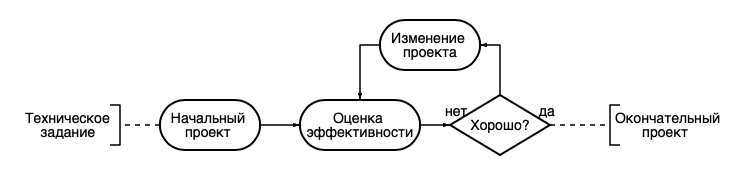
\includegraphics[height = 3 cm, keepaspectratio]{../assets/images/1_1_1diagram.png}
		\caption{ Процесс оптимизации }
		\label{fig:diagram_1}
	\end{figure}

Алгоритм оптимизации используется для постепенного улучшения проекта до тех пор, пока проект больше не может быть улучшен или пока не будет затрачено запланированное время либо превышена предельно допустимая стоимость. Конструктор несет ответственность за анализ результатов процесса оптимизации, чтобы обеспечить его пригодность для конечного применения. Неправильные спецификации в постановке задачи, плохой начальный проект и неправильно реализованные или неподходящие алгоритмы оптимизации могут привести к неоптимальным или опасным проектам.

Есть несколько преимуществ оптимизации подхода к проектированию. Прежде всего, процесс оптимизации обеспечивает систематическую, логичную процедуру проектирования. При ее правильном соблюдении алгоритмы оптимизации могут уменьшить вероятность ошибки человека при проектировании. Интуиция в инженерном проектировании может ввести в заблуждение; намного лучше оптимизировать данные. Оптимизация может ускорить процесс проектирования, особенно когда процедура может быть написана один раз, а затем повторно применена к другим задачам. Традиционные инженерные методы часто визуализируются и обосновываются людьми в двух или трех измерениях. B то же время современные методы оптимизации могут применяться к задачам с миллионами переменных и ограничений.
   
Есть также проблемы, связанные с использованием оптимизации для проектирования. Мы обычно ограничены в наших вычислительных ресурсах и времени, и поэтому наши алгоритмы должны быть избирательными в том, как они исследуют пространство проектных параметров. По сути, алгоритмы оптимизации ограничены способностью конструктора формулировать задачу. B некоторых случаях алгоритм оптимизации может использовать ошибки моделирования или найти решение, которое не позволяет адекватно решить поставленную задачу. Когда алгоритм приводит к оптимальному проекту, который противоречит интуиции, его может быть трудно интерпретировать. Другое ограничение заключается в том, что многие алгоритмы оптимизации не всегда гарантируют получение оптимальных проектов. 

\section{Математическое определение задачи оптимизации}

Основная задача оптимизации формулируется следующим образом:

\begin{equation}
  \min_{x} \, f(x)
  \label{eq:taskOptimizationMin}
\end{equation}

\begin{center}
при условии, что $x \in X$
\end{center}

Здесь $x$ — расчетная точка (design point). Расчетная точка мохет быть представлена как вектор значений, соответствующих различным расчетным переменным (design variables). Расчетная точка в $n$-мерном пространстве записывается следующим образом:

\begin{equation}
    [x_1,x_2,...,x_n],
	\label{eq:arrayX}
\end{equation}

где $i$-я расчетная переменная обозначена $x_i$. Элементы в этом векторе можно регулировать, чтобы минимизировать целевую функцию $f$. Любое значение $x$ из всех точек в допустимом множестве $F$, которое минимизирует целевую функцию, называется решением или точкой минимума. Конкретное решение записывается как $x^*$. Пример задачи одномерной оптимизации показан на рис. \ref{fig:figure_1}

\begin{figure}[ht]
 \centering
		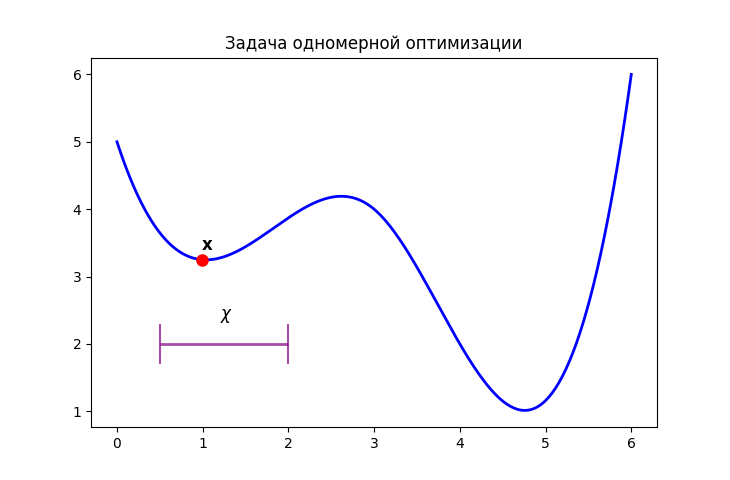
\includegraphics[height =7 cm, keepaspectratio]{../assets/images/Figure_1.png}
		\caption{Минимум является лучшим вариантом в возможном наборе —
вне допустимой области могут существовать точки с более низкими значениями
}
\label{fig:figure_1}
	\end{figure}

Эта формулировка является общей, т.е. любая задача оптимизации может быть переписана в соответствии с уравнением \eqref{eq:taskOptimizationMin}. B частности, задачу

\begin{equation}
  \min_{x} \, f(x) 
\end{equation}

\begin{center}
при условии, что $x \in X$
\end{center}

можно переформулировать так:

\begin{equation}
  \max_{x} \, -f(x) 
  \label{eq:TaskOptimizationMax}
\end{equation}

 \begin{center}
 при условии, что $x \in X$
 \end{center}
 
Задача в новой формулировке имеет тот же самый набор решений. Моделирование инженерных задач в рамках этой математической формулировки может быть сложной задачей. То, как формулируется задача оптимизации, может сделать процесс решения простым или сложным. Следует задаться вопросом какой алгоритм лучше. Если один алгоритм работает лучше, чем другой алгоритм для одного класса задач, то он будет работать хуже для другого класса задач. Чтобы многие алгоритмы оптимизации работали эффективно, в целевой функции должна быть некоторая регулярность, например липшиц-непрерывность или выпуклость. 

\section{Ограничения}

Многие задачи имеют ограничения. Каждое ограничение выделяет множество возможных решений, и в совокупности ограничения определяют допустимое множество  $F$. Допустимые расчетные точки не нарушают никаких ограничений. Например, рассмотрим следующую проблему оптимизации:

\begin{equation}
\min_{x_1, x_2} f(x_1, x_2)
\label{eq:taskOptimizationX1X2}
\end{equation}


 \begin{center}
 при условии, что 
\begin{equation}
  \begin{aligned}
    x_1 &\geq  \\
    x_2 &\geq 0  \\
    x_1 + x_2 &\leq 1
  \end{aligned}
  \label{eq:inequalities}
\end{equation}
\end{center}

Допустимое множество изображено на рис. \ref{fig:figure_2}

\begin{figure}[ht]
 \centering
		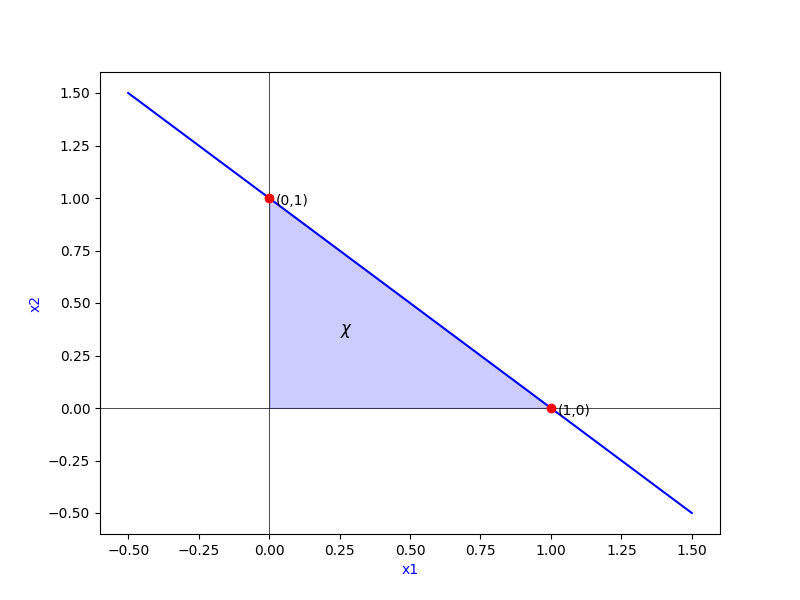
\includegraphics[height = 7 cm, keepaspectratio]{../assets/images/Figure_2.png}
		\caption{Допустимое множество F, заданное неравенствами \eqref{eq:inequalities}}
		\label{fig:figure_2}
	\end{figure}
    
Ограничения обычно записываются с помощью знаков $\leq$, $\geq$ или $=$. Если ограничения включают знаки $<$ или $>$ (т.е. строгие неравенства), то допустимое множество не включает границу ограничений. Потенциальная проблема, которая может возникнуть без учета границы иллюстрируется следующей задачей:


\begin{equation}
  \min_{x} \, x 
  \label{eq:taskOptimizationMin1}
\end{equation}

 \begin{center}
 при условии, что $x>1$
 \end{center}

 Допустимое множество показано на рис. \ref{fig:figure_3} Точка $x = 1$ меньше любого $x$, превышающего единицу, но значение $x = 1$ недопустимо. Можно выбрать любой $x$, произвольно близкий к единице, но превышающей ее, и независимо от того, что выбирать, всегда можно найти бесконечное количество значений, которые расположены еще ближе к единице. Необходимо констатировать, что задача не имеет решения. Чтобы избежать таких проблем, часто лучше включать границу ограничений в допустимое множество.


\begin{figure}[ht]
 \centering
		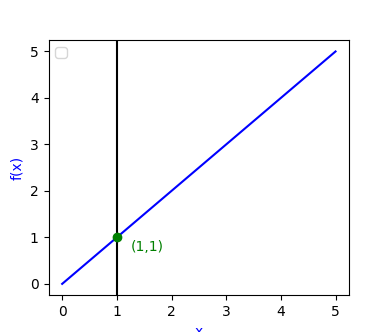
\includegraphics[height = 5 cm, keepaspectratio]{../assets/images/Figure_3.png}
		\caption{ Задача \eqref{eq:taskOptimizationMin1} не имеет решения, поскольку граница ограничения недопустима }
		\label{fig:figure_3}
	\end{figure}
    
\section{Критические точки}

На рис. 2.4.1 ~\ref{fig:figure_4} показана одномерная функция $f(x)$ с несколькими помеченными критическими точками, в которых производная равна нулю и которые представляют интерес при обсуждении задач оптимизации. При минимизации функции $f$ желательно найти точку глобального минимума, т.е. значение $x$, в котором значение $f(x)$ является минимальным. Функция может иметь не более одного глобального минимума, но может иметь несколько точек глобального минимума.

Как правило, трудно доказать, что данная точка-кандидат является точкой глобального минимума. Часто лучшее, что можно сделать, это проверить, соответствует ли она локальному минимуму. Точка $x^*$ является точкой локального минимума, если существует число $\delta > 0$ такое, что $f(x^*) \leq f(x)$ для всех $x$, удовлетворяющих условию $| x - x^*| < \delta$. B многомерном контексте это определение сводится к существованию числа $\delta > 0$ такого, что $f(x^*) \leq f (x)$ для всех $x$, удовлетворяющих условию $||x - x^*|| < \delta$.
На рис. \ref{fig:figure_4} показаны два типа локальных минимумов: сильный и слабый. Точка сильного локального минимума, которая также называется точкой строгого локального минимума, — это точка, которая однозначно минимизирует $f$ в окрестности. Иначе говоря, точка $x^*$ является точкой строгого локального минимума, если существует число $\delta > 0$ такое, что $f(x^*) < f(x)$ всякий раз, когда $x^* \neq x$ и $||x - x^*|| < \delta$. B многомерном контексте это определение сводится к существованию числа $\delta > 0$ такого, что $f(x^*)< f(x)$всякийраз,когда $x^* \neq x$ и $||x - x^*||< \delta$. Точка слабого локального минимума — это точка локального минимума, которая не является точкой сильного локального минимума.

\begin{figure}[ht]
 \centering
		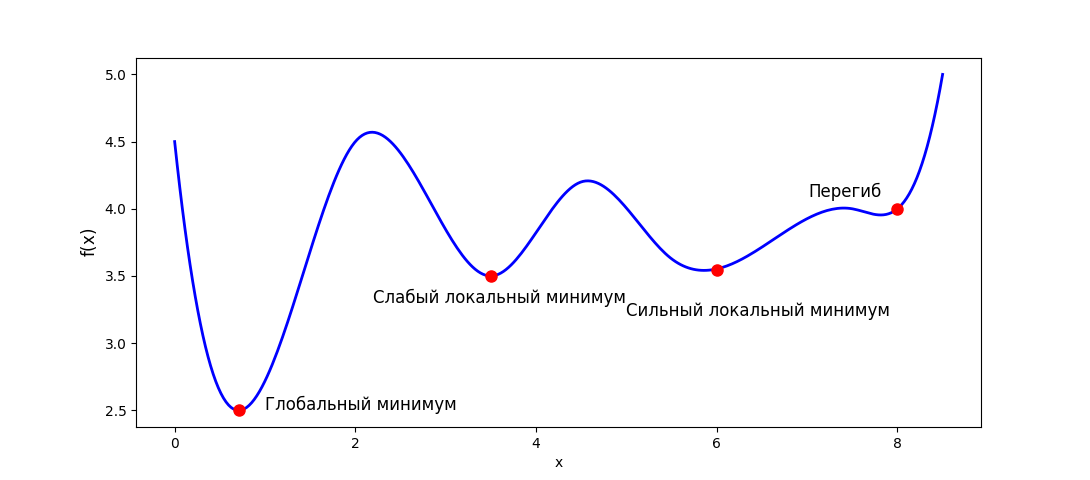
\includegraphics[height =5 cm, keepaspectratio]{../assets/images/Figure_4.png}
		\caption{Примеры критических точек одномерной функции, представляющих интерес для алгоритмов оптимизации (в которых производная равна нулю)
		\label{fig:figure_4}
 }
	\end{figure}
    
Bо всех точках локального и глобального минимума производная непрерывной неограниченной целевой функции равна нулю. Равенство производной нулю — необходимое, но не достаточное условие для локального минимума.
На рис. \ref{fig:figure_4} показана точка перегиба, где производная равна нулю, но эта точка не является точкой локального минимума функции $f$. Точка перегиба — это место, где меняется знак второй производной функции $f$, что соответствует локальному минимуму или максимуму ее первой производной $f '$. Производная в точке перегиба не обязательно равна нулю.

\chapter{ ГЛАВА 2. Задача оптимизации}
\label{ch:chapter2}

\section{Процесс оптимизации}

Многие научные и инженерные дисциплины основаны на оптимизации. B физике системы стремятся к состоянию с наименьшей энергией в соответствии с законами природы. B бизнесе корпорации нацелены на максимальную стоимость акций. B биологии с большей вероятностью выживают более адаптивные организмы. Данная работа посвящена оптимизации с инженерной точки зрения, для которой целью является разработка системы, оптимизирующих набор показателей с учетом ограничений.

Типичный процесс оптимизации инженерного проектирования показан на рис. \ref{fig:diagram_1} Роль конструктора заключается в предоставлении технического задания, которое детализирует параметры, константы, цели и ограничения. Конструктор отвечает за постановку задачи и количественную оценку достоинств потенциальных проектов. Он также обычно предоставляет базовый проект или начальную точку проектирования для алгоритма оптимизации.

\begin{figure}[ht]
 \centering
		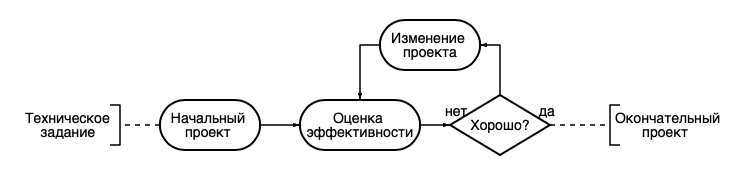
\includegraphics[height = 3 cm, keepaspectratio]{../assets/images/1_1_1diagram.png}
		\caption{ Процесс оптимизации }
		\label{fig:diagram_1}
	\end{figure}

Алгоритм оптимизации используется для постепенного улучшения проекта до тех пор, пока проект больше не может быть улучшен или пока не будет затрачено запланированное время либо превышена предельно допустимая стоимость. Конструктор несет ответственность за анализ результатов процесса оптимизации, чтобы обеспечить его пригодность для конечного применения. Неправильные спецификации в постановке задачи, плохой начальный проект и неправильно реализованные или неподходящие алгоритмы оптимизации могут привести к неоптимальным или опасным проектам.

Есть несколько преимуществ оптимизации подхода к проектированию. Прежде всего, процесс оптимизации обеспечивает систематическую, логичную процедуру проектирования. При ее правильном соблюдении алгоритмы оптимизации могут уменьшить вероятность ошибки человека при проектировании. Интуиция в инженерном проектировании может ввести в заблуждение; намного лучше оптимизировать данные. Оптимизация может ускорить процесс проектирования, особенно когда процедура может быть написана один раз, а затем повторно применена к другим задачам. Традиционные инженерные методы часто визуализируются и обосновываются людьми в двух или трех измерениях. B то же время современные методы оптимизации могут применяться к задачам с миллионами переменных и ограничений.
   
Есть также проблемы, связанные с использованием оптимизации для проектирования. Мы обычно ограничены в наших вычислительных ресурсах и времени, и поэтому наши алгоритмы должны быть избирательными в том, как они исследуют пространство проектных параметров. По сути, алгоритмы оптимизации ограничены способностью конструктора формулировать задачу. B некоторых случаях алгоритм оптимизации может использовать ошибки моделирования или найти решение, которое не позволяет адекватно решить поставленную задачу. Когда алгоритм приводит к оптимальному проекту, который противоречит интуиции, его может быть трудно интерпретировать. Другое ограничение заключается в том, что многие алгоритмы оптимизации не всегда гарантируют получение оптимальных проектов. 

\section{Математическое определение задачи оптимизации}

Основная задача оптимизации формулируется следующим образом:

\begin{equation}
  \min_{x} \, f(x)
  \label{eq:taskOptimizationMin}
\end{equation}

\begin{center}
при условии, что $x \in X$
\end{center}

Здесь $x$ — расчетная точка (design point). Расчетная точка мохет быть представлена как вектор значений, соответствующих различным расчетным переменным (design variables). Расчетная точка в $n$-мерном пространстве записывается следующим образом:

\begin{equation}
    [x_1,x_2,...,x_n],
	\label{eq:arrayX}
\end{equation}

где $i$-я расчетная переменная обозначена $x_i$. Элементы в этом векторе можно регулировать, чтобы минимизировать целевую функцию $f$. Любое значение $x$ из всех точек в допустимом множестве $F$, которое минимизирует целевую функцию, называется решением или точкой минимума. Конкретное решение записывается как $x^*$. Пример задачи одномерной оптимизации показан на рис. \ref{fig:figure_1}

\begin{figure}[ht]
 \centering
		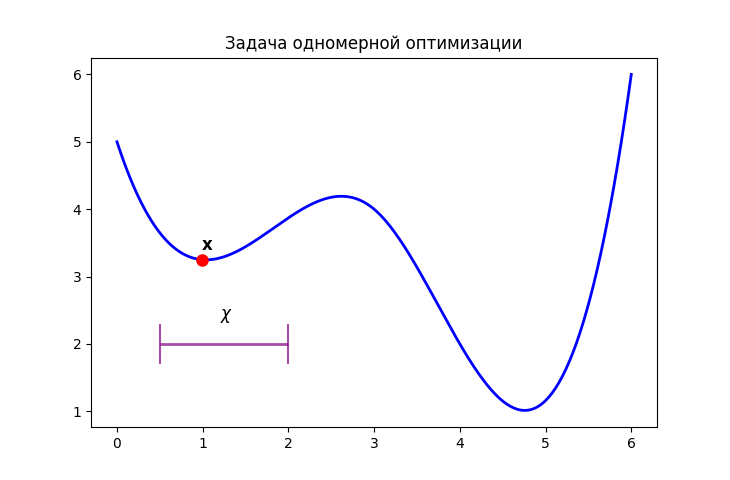
\includegraphics[height =7 cm, keepaspectratio]{../assets/images/Figure_1.png}
		\caption{Минимум является лучшим вариантом в возможном наборе —
вне допустимой области могут существовать точки с более низкими значениями
}
\label{fig:figure_1}
	\end{figure}

Эта формулировка является общей, т.е. любая задача оптимизации может быть переписана в соответствии с уравнением \eqref{eq:taskOptimizationMin}. B частности, задачу

\begin{equation}
  \min_{x} \, f(x) 
\end{equation}

\begin{center}
при условии, что $x \in X$
\end{center}

можно переформулировать так:

\begin{equation}
  \max_{x} \, -f(x) 
  \label{eq:TaskOptimizationMax}
\end{equation}

 \begin{center}
 при условии, что $x \in X$
 \end{center}
 
Задача в новой формулировке имеет тот же самый набор решений. Моделирование инженерных задач в рамках этой математической формулировки может быть сложной задачей. То, как формулируется задача оптимизации, может сделать процесс решения простым или сложным. Следует задаться вопросом какой алгоритм лучше. Если один алгоритм работает лучше, чем другой алгоритм для одного класса задач, то он будет работать хуже для другого класса задач. Чтобы многие алгоритмы оптимизации работали эффективно, в целевой функции должна быть некоторая регулярность, например липшиц-непрерывность или выпуклость. 

\section{Ограничения}

Многие задачи имеют ограничения. Каждое ограничение выделяет множество возможных решений, и в совокупности ограничения определяют допустимое множество  $F$. Допустимые расчетные точки не нарушают никаких ограничений. Например, рассмотрим следующую проблему оптимизации:

\begin{equation}
\min_{x_1, x_2} f(x_1, x_2)
\label{eq:taskOptimizationX1X2}
\end{equation}


 \begin{center}
 при условии, что 
\begin{equation}
  \begin{aligned}
    x_1 &\geq  \\
    x_2 &\geq 0  \\
    x_1 + x_2 &\leq 1
  \end{aligned}
  \label{eq:inequalities}
\end{equation}
\end{center}

Допустимое множество изображено на рис. \ref{fig:figure_2}

\begin{figure}[ht]
 \centering
		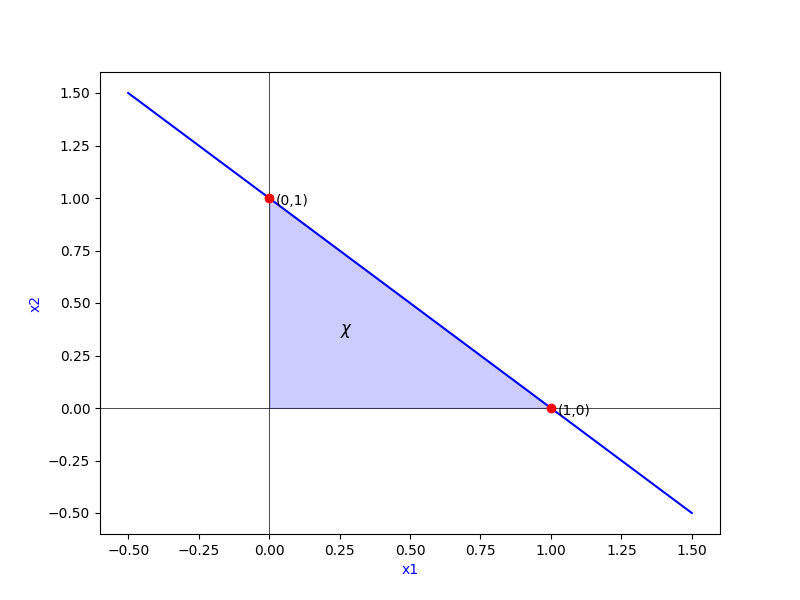
\includegraphics[height = 7 cm, keepaspectratio]{../assets/images/Figure_2.png}
		\caption{Допустимое множество F, заданное неравенствами \eqref{eq:inequalities}}
		\label{fig:figure_2}
	\end{figure}
    
Ограничения обычно записываются с помощью знаков $\leq$, $\geq$ или $=$. Если ограничения включают знаки $<$ или $>$ (т.е. строгие неравенства), то допустимое множество не включает границу ограничений. Потенциальная проблема, которая может возникнуть без учета границы иллюстрируется следующей задачей:


\begin{equation}
  \min_{x} \, x 
  \label{eq:taskOptimizationMin1}
\end{equation}

 \begin{center}
 при условии, что $x>1$
 \end{center}

 Допустимое множество показано на рис. \ref{fig:figure_3} Точка $x = 1$ меньше любого $x$, превышающего единицу, но значение $x = 1$ недопустимо. Можно выбрать любой $x$, произвольно близкий к единице, но превышающей ее, и независимо от того, что выбирать, всегда можно найти бесконечное количество значений, которые расположены еще ближе к единице. Необходимо констатировать, что задача не имеет решения. Чтобы избежать таких проблем, часто лучше включать границу ограничений в допустимое множество.


\begin{figure}[ht]
 \centering
		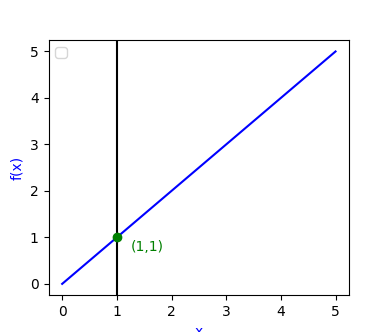
\includegraphics[height = 5 cm, keepaspectratio]{../assets/images/Figure_3.png}
		\caption{ Задача \eqref{eq:taskOptimizationMin1} не имеет решения, поскольку граница ограничения недопустима }
		\label{fig:figure_3}
	\end{figure}
    
\section{Критические точки}

На рис. 2.4.1 ~\ref{fig:figure_4} показана одномерная функция $f(x)$ с несколькими помеченными критическими точками, в которых производная равна нулю и которые представляют интерес при обсуждении задач оптимизации. При минимизации функции $f$ желательно найти точку глобального минимума, т.е. значение $x$, в котором значение $f(x)$ является минимальным. Функция может иметь не более одного глобального минимума, но может иметь несколько точек глобального минимума.

Как правило, трудно доказать, что данная точка-кандидат является точкой глобального минимума. Часто лучшее, что можно сделать, это проверить, соответствует ли она локальному минимуму. Точка $x^*$ является точкой локального минимума, если существует число $\delta > 0$ такое, что $f(x^*) \leq f(x)$ для всех $x$, удовлетворяющих условию $| x - x^*| < \delta$. B многомерном контексте это определение сводится к существованию числа $\delta > 0$ такого, что $f(x^*) \leq f (x)$ для всех $x$, удовлетворяющих условию $||x - x^*|| < \delta$.
На рис. \ref{fig:figure_4} показаны два типа локальных минимумов: сильный и слабый. Точка сильного локального минимума, которая также называется точкой строгого локального минимума, — это точка, которая однозначно минимизирует $f$ в окрестности. Иначе говоря, точка $x^*$ является точкой строгого локального минимума, если существует число $\delta > 0$ такое, что $f(x^*) < f(x)$ всякий раз, когда $x^* \neq x$ и $||x - x^*|| < \delta$. B многомерном контексте это определение сводится к существованию числа $\delta > 0$ такого, что $f(x^*)< f(x)$всякийраз,когда $x^* \neq x$ и $||x - x^*||< \delta$. Точка слабого локального минимума — это точка локального минимума, которая не является точкой сильного локального минимума.

\begin{figure}[ht]
 \centering
		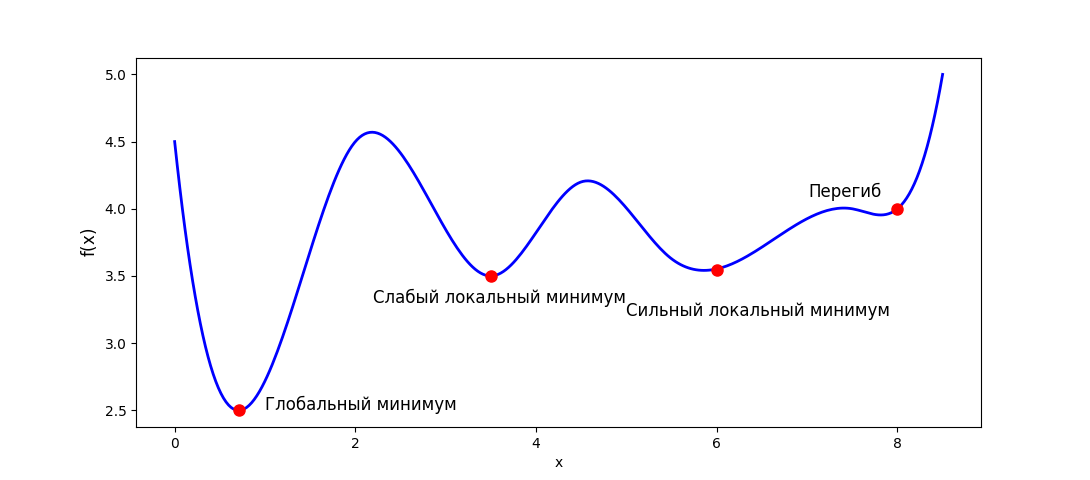
\includegraphics[height =5 cm, keepaspectratio]{../assets/images/Figure_4.png}
		\caption{Примеры критических точек одномерной функции, представляющих интерес для алгоритмов оптимизации (в которых производная равна нулю)
		\label{fig:figure_4}
 }
	\end{figure}
    
Bо всех точках локального и глобального минимума производная непрерывной неограниченной целевой функции равна нулю. Равенство производной нулю — необходимое, но не достаточное условие для локального минимума.
На рис. \ref{fig:figure_4} показана точка перегиба, где производная равна нулю, но эта точка не является точкой локального минимума функции $f$. Точка перегиба — это место, где меняется знак второй производной функции $f$, что соответствует локальному минимуму или максимуму ее первой производной $f '$. Производная в точке перегиба не обязательно равна нулю.

\chapter{Реализация модели в Timefold Solver}
\label{ch:chapter3}

\section{Архитектура и ключевые понятия Timefold Solver}

Для решения задачи оптимизации упаковки сырков была выбрана библиотека Timefold Solver — современный инструмент с открытым исходным кодом, предназначенный для построения оптимальных расписаний и планов. Timefold продолжает развитие библиотеки OptaPlanner и ориентирован на использование в производственных системах, логистике, управлении ресурсами и других сферах, где критически важны точность и эффективность планирования. Библиотека реализует мощные метаэвристики, такие как Late Acceptance, Simulated Annealing, Tabu Search, а также предоставляет удобный способ моделирования задачи через аннотированные Java-классы.

Timefold активно используется в таких сценариях, как производственное планирование, создание сменных расписаний для сотрудников, маршрутизация транспорта, автоматизация логистики, оптимизация загрузки станков и, в рамках данной работы, — организация процессов фасовки пищевых продуктов. Благодаря гибкой архитектуре и высокой расширяемости, Timefold подходит как для малых предприятий, так и для сложных промышленных систем с тысячами объектов и ограничений.

Процесс планирования в Timefold условно делится на несколько ключевых этапов. На первом этапе выполняется моделирование задачи, в ходе которого описываются основные компоненты модели. Классы, изменяемые во время решения задачи, аннотируются как @PlanningEntity, и в них указываются переменные, которые будут подбираться планировщиком — например, назначение линии фасовки или временного слота. Эти переменные отмечаются аннотацией @PlanningVariable. Главный класс, содержащий всё решение, включая список сущностей, фиксированные данные (например, список линий или продуктов), а также итоговый score, аннотируется как @PlanningSolution.

После описания структуры задачи создаются ограничения, определяющие допустимые и желаемые состояния решения. Для этого используется класс ConstraintProvider, реализующий интерфейс ConstraintProvider и переопределяющий метод defineConstraints. В этом методе на языке Java (с использованием Constraint Streams API) задаются логические правила, штрафы и бонусы за выполнение или нарушение определённых условий, таких как: необходимость мойки между аллергенами, минимальная загрузка линии, максимальная производительность и др.

После моделирования задачи происходит инициализация решателя, где считывается конфигурация из XML-файла или с помощью Java DSL. Конфигурация определяет, какие фазы оптимизации использовать, какие метаэвристики активировать, сколько времени выделить на решение задачи и как реагировать на новые входные данные. После запуска планировщик загружает исходное решение, допустимые значения переменных, и начинает подбор решения.

На первой фазе работает Construction Heuristics — она быстро формирует первое допустимое, но не обязательно оптимальное решение. Это решение служит отправной точкой для дальнейшего улучшения. Например, фасовочные задания могут быть распределены по линиям произвольно или с минимальным количеством нарушений, но без учёта всех ограничений.

Затем запускается фаза Local Search, во время которой происходит пошаговое улучшение решения с применением метаэвристик. На каждом шаге планировщик выбирает возможный ход (изменение одной или нескольких переменных), пересчитывает значение score, и на основе используемой стратегии решает, принять ли новое решение. Например, стратегия Simulated Annealing может временно принять ухудшенное решение, чтобы избежать локального оптимума. Процесс продолжается до достижения заданного лимита по времени, шагам или качеству.

Результат работы решателя — это оптимизированное расписание, которое может быть отображено пользователю через визуализацию, сохранено в базе данных или экспортировано для дальнейшей интеграции с другими системами.

Timefold предоставляет множество аннотаций, играющих ключевую роль в описании модели. Рассмотрим основные из них:

@PlanningSolution — аннотация, указывающая, что данный класс является корневым элементом решения. Он содержит список сущностей (@PlanningEntity), фактов (@ProblemFact), конфигурацию и score (результат оценки качества решения).

@PlanningEntity — используется для классов, переменные которых будут изменяться во время оптимизации. Например, в задаче фасовки — это задания (Jobs), которые могут быть перемещены между линиями, а также иметь различные временные слоты.

@PlanningVariable — помечает поле внутри сущности, которое будет оптимизироваться решателем. Обязательно указывается valueRangeProviderRefs, ссылающийся на метод или поле, предоставляющее допустимые значения переменной. Например, список всех доступных линий фасовки.

@ValueRangeProvider — аннотация, предоставляющая набор допустимых значений для @PlanningVariable. Может быть объявлена в корневом классе решения или отдельном компоненте.

@ProblemFact и @ProblemFactCollectionProperty — применяются для неизменяемых данных, используемых при расчётах и в ограничениях. Это, например, список производственных линий, типов продукции, скорости работы линий, санитарные интервалы и т.д. Эти данные не изменяются решателем, но активно используются в логике ограничения.

@ShadowVariable — особая аннотация для переменных, которые вычисляются автоматически на основе других переменных. Shadow-переменные не подбираются решателем напрямую, но их значения важны для ограничения и отображения. Примеры: endTime = startTime + duration, где duration может зависеть от типа продукта и линии.

@CascadingShadowVariable — указывает, что изменение одной переменной должно инициировать пересчёт других связанных shadow-переменных. Например, если меняется назначение линии, автоматически пересчитывается скорость фасовки, а затем — длительность и время окончания.

Timefold Solver предоставляет мощные механизмы для построения гибких и расширяемых моделей. Одной из ключевых особенностей является его способность использовать декларативные ограничения, которые можно динамически включать или отключать, управлять приоритетами, а также отслеживать влияние каждого ограничения на итоговый score. Это даёт разработчику возможность точно настраивать поведение планировщика под конкретные бизнес-цели.

В сочетании с современными фреймворками, такими как Quarkus, Spring Boot или Micronaut, Timefold позволяет строить масштабируемые приложения для производственного планирования, интегрированные с базами данных, REST-интерфейсами и визуализациями. Такая архитектура обеспечивает высокую гибкость, расширяемость и удобство сопровождения производственных ИИ-систем.

\section{Описание реализации}

Для реализации программной части проекта был выбран язык программирования \textbf{Java}. Этот выбор обусловлен несколькими ключевыми факторами. Во-первых, Java является одним из наиболее распространённых и зрелых языков в области корпоративной разработки, обладающим широкой экосистемой библиотек и фреймворков. Во-вторых, Timefold Solver, который используется в данном проекте в качестве ядра для оптимизации, предоставляет официальный API на Java, что обеспечивает естественную и эффективную интеграцию с решателем. Благодаря строгой типизации и развитой системе обработки исключений Java способствует созданию надёжного и масштабируемого кода, что особенно важно при реализации сложных алгоритмов планирования и бизнес-логики.

Для управления проектом и автоматизации процессов сборки, тестирования и деплоя была использована система сборки \textbf{Apache Maven}. Maven позволяет определить структуру проекта, зависимости и плагины через декларативный файл конфигурации \texttt{pom.xml}, что упрощает поддержку и развитие программного обеспечения. В рамках проекта Maven отвечает за загрузку всех необходимых библиотек (например, Timefold Solver, библиотеки для работы с REST API и др.), компиляцию исходного кода, запуск тестов и упаковку приложения.

Основным преимуществом использования Maven является стандартизация процесса сборки, что позволяет новым разработчикам быстро войти в проект, а также легко интегрировать приложение с системами непрерывной интеграции и развёртывания (CI/CD). Кроме того, благодаря центральному репозиторию Maven разработчики могут оперативно получать обновления библиотек и обеспечивать совместимость версий.

Для удобства разработки и отладки на локальной машине применяется команда

\begin{verbatim}
mvn clean quarkus:dev
\end{verbatim}

Эта команда выполняет несколько последовательных действий:

\begin{itemize}
    \item \texttt{clean} — очищает предыдущие результаты сборки, удаляя папку \texttt{target}, где Maven хранит скомпилированные классы и артефакты. Это гарантирует, что сборка будет выполнена «с нуля», без влияния старых файлов.
    \item \texttt{quarkus:dev} — запускает приложение в режиме «горячей» перезагрузки (hot reload), предоставляемом фреймворком Quarkus. Этот режим позволяет разработчику вносить изменения в код и видеть их результат без необходимости перезапуска сервера. Это существенно ускоряет цикл разработки и отладки.
\end{itemize}

Quarkus — современный Java-фреймворк, ориентированный на создание высокопроизводительных микросервисов и облачных приложений с минимальным временем запуска и низким потреблением ресурсов. В проекте Quarkus используется для реализации REST API и взаимодействия между компонентами системы, а также для интеграции с Timefold Solver.

Сочетание Java, Maven и Quarkus обеспечивает удобную, эффективную и масштабируемую платформу для реализации системы оптимизации фасовочных линий, позволяя гибко настраивать бизнес-логику и оперативно реагировать на изменения требований.

\section{Как работает планировщик}

В рамках построения системы оптимизации фасовки продукции ключевую роль играют классы, аннотированные как \texttt{@PlanningEntity}. Это сущности, изменяемые в процессе решения задачи, значения которых подбирает планировщик Timefold. В данной модели такими сущностями являются классы \texttt{Job} и \texttt{Line}. Оба класса участвуют в построении расписания: \texttt{Job} — это задания, которые необходимо распределить между линиями фасовки и отсортировать во времени, а \texttt{Line} — объекты, содержащие списки этих заданий, отражающие их последовательность исполнения.

\subsection*{Класс Job — производственный заказ}

Класс \texttt{Job} представляет собой единичное производственное задание: упаковку заданного количества конкретного продукта на одной из фасовочных линий. Именно объекты этого класса перемещаются планировщиком между линиями и позициями в цепочке заданий.

Каждое задание включает в себя уникальный идентификатор (\texttt{id}) и наименование (\texttt{name}) для удобства идентификации и отображения. Важнейшим свойством \texttt{Job} является объект \texttt{Product}, указывающий на упаковываемый продукт, с его характеристиками: тип, категория, наличие аллергенов, тип глазури и др.

Также \texttt{Job} содержит информацию о требуемом объёме фасовки (\texttt{quantity}) и продолжительности выполнения (\texttt{duration}). В некоторых случаях \texttt{duration} может задаваться явно, но чаще всего она рассчитывается автоматически на основе скорости линии и количества продукции — это делается с помощью \texttt{@ShadowVariable}.

Особое значение имеют временные ограничения:
\begin{itemize}
    \item \texttt{minStartTime} — минимально допустимое время начала задания;
    \item \texttt{idealEndTime} — желаемое время завершения (используется для мягких ограничений);
    \item \texttt{maxEndTime} — крайний срок завершения (жёсткое ограничение).
\end{itemize}

Поле \texttt{priority} определяет относительную важность задания, что влияет на предпочтения планировщика при выборе порядка исполнения.

Аннотация \texttt{@PlanningPin} используется для фиксации некоторых заданий — такие объекты не будут изменяться решателем. Это может быть полезно для ручных корректировок или защиты утверждённых операций.

Наконец, класс \texttt{Job} хранит ссылки на текущую назначенную линию (\texttt{line}), а также на предыдущие и последующие задания в цепочке (\texttt{previousJob}, \texttt{nextJob}). Это необходимо для реализации chain-based модели — подхода, при котором задания на линии образуют связанную последовательность, важную для соблюдения технологических ограничений (например, мойка между несовместимыми продуктами).

\begin{lstlisting}[caption={Класс Job}, label={lst:classJob}]
@PlanningEntity
public class Job {
    @PlanningId
    private String id;
    private String name;
    private Product product;
    private int quantity;
    private Duration duration;
    private LocalDateTime minStartTime;
    private LocalDateTime idealEndTime;
    private LocalDateTime maxEndTime;
    private int priority;
    @PlanningPin
    private boolean pinned;

    @PlanningVariable(...)
    private Line line;

    @PreviousElementShadowVariable(...)
    private Job previousJob;

    @NextElementShadowVariable(...)
    private Job nextJob;

    @ShadowVariable(...)
    private LocalDateTime startCleaningDateTime;

    @ShadowVariable(...)
    private LocalDateTime startProductionDateTime;

    @ShadowVariable(...)
    private LocalDateTime endDateTime;

    ...
}
\end{lstlisting}

Важной частью логики \texttt{Job} являются shadow-поля, автоматически пересчитываемые планировщиком при изменении основной переменной. Например, \texttt{startCleaningDateTime} зависит от предыдущего задания, а также от длительности мойки между типами продуктов. Это поведение реализуется через аннотацию \texttt{@CascadingShadowVariable}, которая указывает планировщику пересчитывать производные поля при любом изменении ключевых переменных (линии или позиции в цепочке).

Таким образом, \texttt{Job} — это основной объект, перемещаемый как по временной шкале, так и между линиями. Timefold подбирает наиболее подходящее назначение (\texttt{line}) и позицию в последовательности (через список \texttt{jobs} в \texttt{Line}), стремясь минимизировать общие потери времени, избежать пересечений и удовлетворить всем заданным ограничениям.

\subsection*{Класс Line — фасовочная линия}

Класс \texttt{Line} представляет собой производственную линию, на которую назначаются задания типа \texttt{Job}. Несмотря на то, что сама линия, как правило, не изменяется во время оптимизации, она аннотируется как \texttt{@PlanningEntity}, поскольку содержит переменную планирования — список заданий \texttt{jobs}.

Каждая линия имеет уникальные атрибуты: идентификатор (\texttt{id}), название (\texttt{name}), имя оператора (\texttt{operator}) и стартовое время (\texttt{startDateTime}), указывающее, когда может начаться первый процесс фасовки на данной линии. Однако ключевым элементом класса является поле:

\begin{lstlisting}[caption={Класс Line}, label={lst:classLine}]
@PlanningEntity
public class Line {
    @PlanningId
    private String id;
    private String name;
    private String operator;
    private LocalDateTime startDateTime;

    @JsonIgnore
    @PlanningListVariable
    private List<Job> jobs;
    ...
}
\end{lstlisting}

Аннотация \texttt{@PlanningListVariable} сообщает планировщику, что \texttt{jobs} является переменной, подлежащей изменению. Timefold будет перемещать объекты \texttt{Job} между списками различных линий и менять их порядок, тем самым формируя расписание.

Таким образом, модель планирования основана на цепочках: каждый \texttt{Line} содержит последовательность \texttt{Job}, а каждый \texttt{Job} знает своё положение в цепочке через поля \texttt{previousJob} и \texttt{nextJob}. Этот подход облегчает реализацию ограничений, связанных с технологическими переходами, длительностью мойки и управлением временем.

\subsection*{Класс PackagingSchedule — решение задачи планирования}

Центральным элементом задачи является класс \texttt{PackagingSchedule}, помеченный как \texttt{@PlanningSolution}. Это основной контейнер, объединяющий все элементы модели: планируемые сущности, факты задачи, а также результирующий \texttt{score}.

Он включает в себя:

\begin{itemize}
    \item \texttt{workCalendar} — объект, задающий рабочее время и границы планирования;
    \item \texttt{products} — список всех доступных продуктов;
    \item \texttt{lines} — список линий фасовки;
    \item \texttt{jobs} — список заданий, распределяемых между линиями;
    \item \texttt{score} — результат оценки текущего расписания.
\end{itemize}

\begin{lstlisting}[caption={Класс PackagingSchedule}, label={lst:classPackagingSchedule}]
@PlanningSolution
public class PackagingSchedule {

    @ProblemFactProperty
    private WorkCalendar workCalendar;

    @ProblemFactCollectionProperty
    private List<Product> products;

    @PlanningEntityCollectionProperty
    private List<Line> lines;

    @PlanningEntityCollectionProperty
    @ValueRangeProvider
    private List<Job> jobs;

    @PlanningScore
    private HardMediumSoftLongScore score;

    private SolverStatus solverStatus;
    ...
}
\end{lstlisting}

Аннотация \texttt{@ProblemFactProperty} указывает на неизменяемые свойства, которые используются при построении ограничений, но не подлежат изменению во время решения. В данном случае это рабочий календарь (\texttt{workCalendar}) и список продуктов (\texttt{products}).

Поля \texttt{@PlanningEntityCollectionProperty} для \texttt{lines} и \texttt{jobs} означают, что это планируемые сущности: планировщик будет изменять их внутреннее состояние в процессе решения.

Поле \texttt{@PlanningScore} хранит текущую оценку решения. Используется трёхуровневая модель:

\begin{itemize}
    \item \textbf{Hard} — жёсткие ограничения (например, пересечения заданий во времени);
    \item \textbf{Medium} — средние ограничения (например, соблюдение приоритетов);
    \item \textbf{Soft} — мягкие ограничения (например, минимизация простоев).
\end{itemize}

Поле \texttt{solverStatus} не используется самим решателем, но помогает внешним компонентам системы (например, UI) отслеживать состояние оптимизации — работает ли она сейчас или уже завершена.

\vspace{1em}

Таким образом, Timefold формирует расписание, изменяя переменные планирования внутри объектов \texttt{Job}, размещая их в цепочках \texttt{jobs} на линиях \texttt{Line}, соблюдая все ограничения и минимизируя суммарный \texttt{score}. Эта архитектура делает систему гибкой, расширяемой и подходящей для реального производственного применения.

\section{Расчет времени выполнения задач}

Поскольку производственная скорость фасовочных линий существенно различается в зависимости от их типа и особенностей упаковываемого продукта. Для точного расчета времени выполнения задач (jobs) была введена динамическая модель вычисления длительности: фактическое время определяется не заранее, а на этапе планирования, с учётом линии, на которую назначена задача. Однако, с целью оптимизации производительности планировщика, данная динамика применяется не ко всем видам продукции. Например, для типа ROD известно, что он может производиться только на линиях 4, 5 и 6, где производственная скорость идентична — 198 единиц в минуту. Таким образом, длительность задач с таким продуктом можно заранее вычислять по формуле quantity / 198 + 4, без учёта линии. Добавлениия четырех минут к формле расчета обусловлено тем, что может возникнуть необходимость смены пленки на лнии. Аналогично фиксированная скорость используется и для других типов продукции, таких как CACTUS (184 ед/мин) и PLUSH (164 ед/мин), поскольку у них нет значительной зависимости от конкретной линии. Исключение составляет продукция типа CLASSIC, у которой наблюдаются существенные различия: на линии 1 скорость составляет 200, а на линии 6 — 240 сырков в минуту. Для этого случая используется специальный класс DurationProvider, который получает на вход продукт, линию и количество, и возвращает длительность задачи в зависимости от реальной скорости линии. Хотя данный подход универсален и может применяться для всех задач, его использование приводит к увеличению времени расчёта, поэтому он применяется преимущественно для продукции, чувствительной к выбору линии, например, типа CLASSIC.

\vspace{3cm}
\begin{lstlisting}[caption={класс DurationProvider}, label={lst:classDurationProvider}]
public class DurationProvider {
    public Duration calculate(Product product, Line line, int quantity) {
        int speed;

        switch (product.getType()) {
            case PLUSH:
                speed = 164;
                break;
            case CACTUS:
                speed = 184;
                break;
            case ROD:
                speed = 198;
                break;
            case CLASSIC:
                if (line != null && "6".equals(line.getId())) {
                    speed = 240;
                    return Duration.ofMinutes((long)Math.ceil(quantity / (double)speed) + 4);
                } else {
                    speed = 200;
                }
                break;
            default:
                speed = 200;
        }
        return Duration.ofMinutes((long)Math.ceil(quantity / (double)speed) + 4);
    }
}
\end{lstlisting}

\section{Ограничения и ConstraintProvider}

Ограничения (constraints) — это основа работы планировщика Timefold Solver. Они определяют, какие решения считаются допустимыми (жёсткие ограничения) и какие — предпочтительными (мягкие ограничения). Реализация ограничений выполняется в классе, реализующем интерфейс ConstraintProvider.

В данной работе используется класс FoodPackagingConstraintProvider, реализующий интерфейс ConstraintProvider. Метод defineConstraints возвращает массив всех ограничений, разделённых по уровням важности: hard, medium и soft. Оценка расписания производится с использованием трёхуровневого скоринга HardMediumSoftLongScore.

\vspace{5cm}

\begin{lstlisting}[caption={класс FoodPackagingConstraintProvider}, label={lst:classConstraintProvider}]
public class FoodPackagingConstraintProvider implements ConstraintProvider {

    @Override
    public Constraint[] defineConstraints(ConstraintFactory factory) {
        return new Constraint[] {
                // Hard constraints
                maxEndDateTime(factory),
                plushMustBeOnLine1(factory),
                rodOnlyOnLines456(factory),
                cactusOnlyOnLines123(factory),
                classicOnlyOnLines1236(factory),
                // Medium constraints
                idealEndDateTime(factory),
                // Soft constraints
                operatorCleaningConflict(factory),
                minimizeMakespan(factory)
        };
    }
    ...
}
\end{lstlisting}

Жёсткие ограничения (Hard constraints) обязательно должны соблюдаться. Нарушение любого из них делает решение недопустимым.

\begin{itemize}
    \item maxEndDateTime — запрещает завершать работу позже максимально допустимого времени. Штраф пропорционален количеству минут просрочки.
    \item plushMustBeOnLine1 — продукция типа PLUSH может быть упакована только на линии 1.
    \item rodOnlyOnLines456 — продукция типа ROD может быть фасована только на линиях 4, 5 или 6.
    \item cactusOnlyOnLines123 — продукция типа CACTUS допускается к фасовке только на линиях 1, 2 или 3.
    \item classicOnlyOnLines1236 — продукция типа CLASSIC допускается к фасовке только на линиях 1, 2, 3 и 6.
\end{itemize}

Эти ограничения учитывают как бизнес-правила, так и технологические особенности фасовочных линий.

Ограничения средней важности (Medium constraints) влияют на качество решения, но не делают его недопустимым при нарушении. Пример:

idealEndDateTime — желательно, чтобы задание завершилось не позже «идеального» времени (idealEndTime). При нарушении начисляется штраф, пропорциональный количеству минут отклонения.

Это ограничение даёт планировщику гибкость в пределах допустимого окна, улучшая соблюдение предпочтительных сроков.

 Мягкие ограничения (Soft constraints) направлены на улучшение качества решения с точки зрения эффективности и удобства. Пример:

 operatorCleaningConflict — минимизирует конфликты в расписании мойки между заданиями, закреплёнными за одним оператором. Если два задания требуют внимания одного оператора и пересекаются во времени, начисляется штраф за пересечение интервалов между startCleaningDateTime и startProductionDateTime.

 minimizeMakespan — минимизирует общую продолжительность работы линии. Рассчитывается как квадрат времени от начала смены до завершения последнего задания. Это способствует равномерному распределению нагрузки и завершению смен вовремя.

 minimizeCleaningDuration (пока не включено в массив ограничений) — штрафует за чрезмерную длительность промежутков между заданиями, возникающих из-за необходимости санитарной обработки (мойки). Чем выше приоритет задания, тем выше штраф за долгую подготовку к его производству.

 Взаимодействие ограничений.

Ограничения организованы по трём уровням важности, что позволяет Timefold Solver эффективно искать компромиссы:

\begin{itemize}
    \item Нарушения жёстких ограничений полностью исключают решение;
    \item Средние ограничения помогают расставить приоритеты внутри допустимых решений;
    \item Мягкие ограничения способствуют повышению эффективности, снижению издержек и упрощению логистики.
\end{itemize}

Использование Constraint Streams позволяет выразить ограничения декларативно, а не императивно, что упрощает понимание и расширение модели.
\section{Визуализация расписания фасовки с Timefold и Quarkus}

В современных производственных системах для управления процессами фасовки сырков важным аспектом является не только нахождение оптимального расписания, но и его наглядное представление. Для этого в нашем решении используется встроенная визуализация, предоставляемая Timefold Solver. Данная визуализация позволяет в режиме реального времени отслеживать ход работы планировщика, демонстрируя динамическое изменение расписания по мере улучшения решений. Это значительно облегчает анализ и понимание полученных планов, позволяя выявлять узкие места и потенциальные конфликты в производственном процессе.

Визуализация интегрирована в веб-приложение, разработанное с использованием фреймворка Quarkus — современного Java-стека, ориентированного на создание легковесных, высокопроизводительных микросервисов и облачных приложений. Quarkus обеспечивает быстрый старт и низкое потребление ресурсов, что особенно важно для приложений с интерактивным интерфейсом и необходимостью обрабатывать большие объёмы данных в режиме реального времени. Использование аннотаций @QuarkusApplication и @ApplicationScoped позволяет эффективно управлять жизненным циклом компонентов, обеспечивая при этом удобство масштабирования и интеграции с другими сервисами.

Приложение взаимодействует с производственной информационной системой MES через JDBC, загружая демонстрационные данные — сведения о заказах, продуктах, линиях и текущем состоянии производства. Эти данные преобразуются в планировочные сущности, такие как PackagingSchedule, которая служит корневым объектом для дальнейшей работы планировщика Timefold. Сохранение начального решения происходит с помощью вызова repository.write(solution), что обеспечивает постоянное хранение состояния в базе данных и гарантирует возможность последующего анализа и отката при необходимости.

Для взаимодействия с клиентской частью используется современный стек REST и WebSocket. REST API предоставляет интерфейс для загрузки, обновления и получения информации о расписании, а WebSocket обеспечивает двунаправленную связь в реальном времени, позволяя обновлять визуализацию без перезагрузки страницы. Это особенно важно для отображения прогресса планирования и демонстрации изменений расписания по мере работы решателя.

Цикл работы визуализации начинается с загрузки данных из SQL-базы, после чего инициируется процесс оптимизации расписания. Встроенный графический интерфейс Timefold отображает результаты планирования, позволяя пользователю просматривать подробные детали: цепочки заданий, их распределение по линиям, временные интервалы и продолжительность каждой операции. Особое внимание уделяется визуализации очистки линий между сменами продукта — важному этапу, который влияет на производительность и соблюдение санитарных норм.

Основные компоненты визуализации включают в себя несколько ключевых элементов. Задачи (Jobs) представлены в виде прямоугольников, расположенных на временной шкале, где длина каждого блока соответствует времени выполнения задачи. Линии (Lines) отображаются как горизонтальные ряды, каждая из которых соответствует конкретной фасовочной линии на производстве. Временные интервалы, отведённые на мойку оборудования (Cleaning time), выделены отдельными паузами между задачами, что помогает оценить эффективность планирования и соблюдение требований по санитарии.

Кроме того, система визуализации способна подсвечивать нарушения ограничений (Constraints). Например, если между двумя заданиями с разными аллергенами выделено недостаточно времени для полной очистки линии, соответствующий участок визуально отмечается красным или другим цветом предупреждения. Это помогает операторам и инженерам быстро идентифицировать проблемные места и корректировать расписание.

Интеграция Timefold с Quarkus также позволяет легко расширять функциональность визуализации. Благодаря модульности и поддержке стандартных Java-технологий, можно добавлять новые типы ограничений, расширять REST API и улучшать пользовательский интерфейс. Использование Quarkus упрощает развёртывание приложения в контейнерах Docker и облачных платформах, обеспечивая гибкость и масштабируемость решения.

Таким образом, архитектура визуализации расписания фасовки на базе Timefold и Quarkus обеспечивает удобный и эффективный инструмент для мониторинга и анализа производственных процессов. Это позволяет не только находить оптимальные решения, но и быстро их проверять, сравнивать альтернативные варианты и своевременно выявлять потенциальные проблемы, что существенно повышает общую производительность и качество фасовки.
 \begin{figure}[ht]
 \centering
		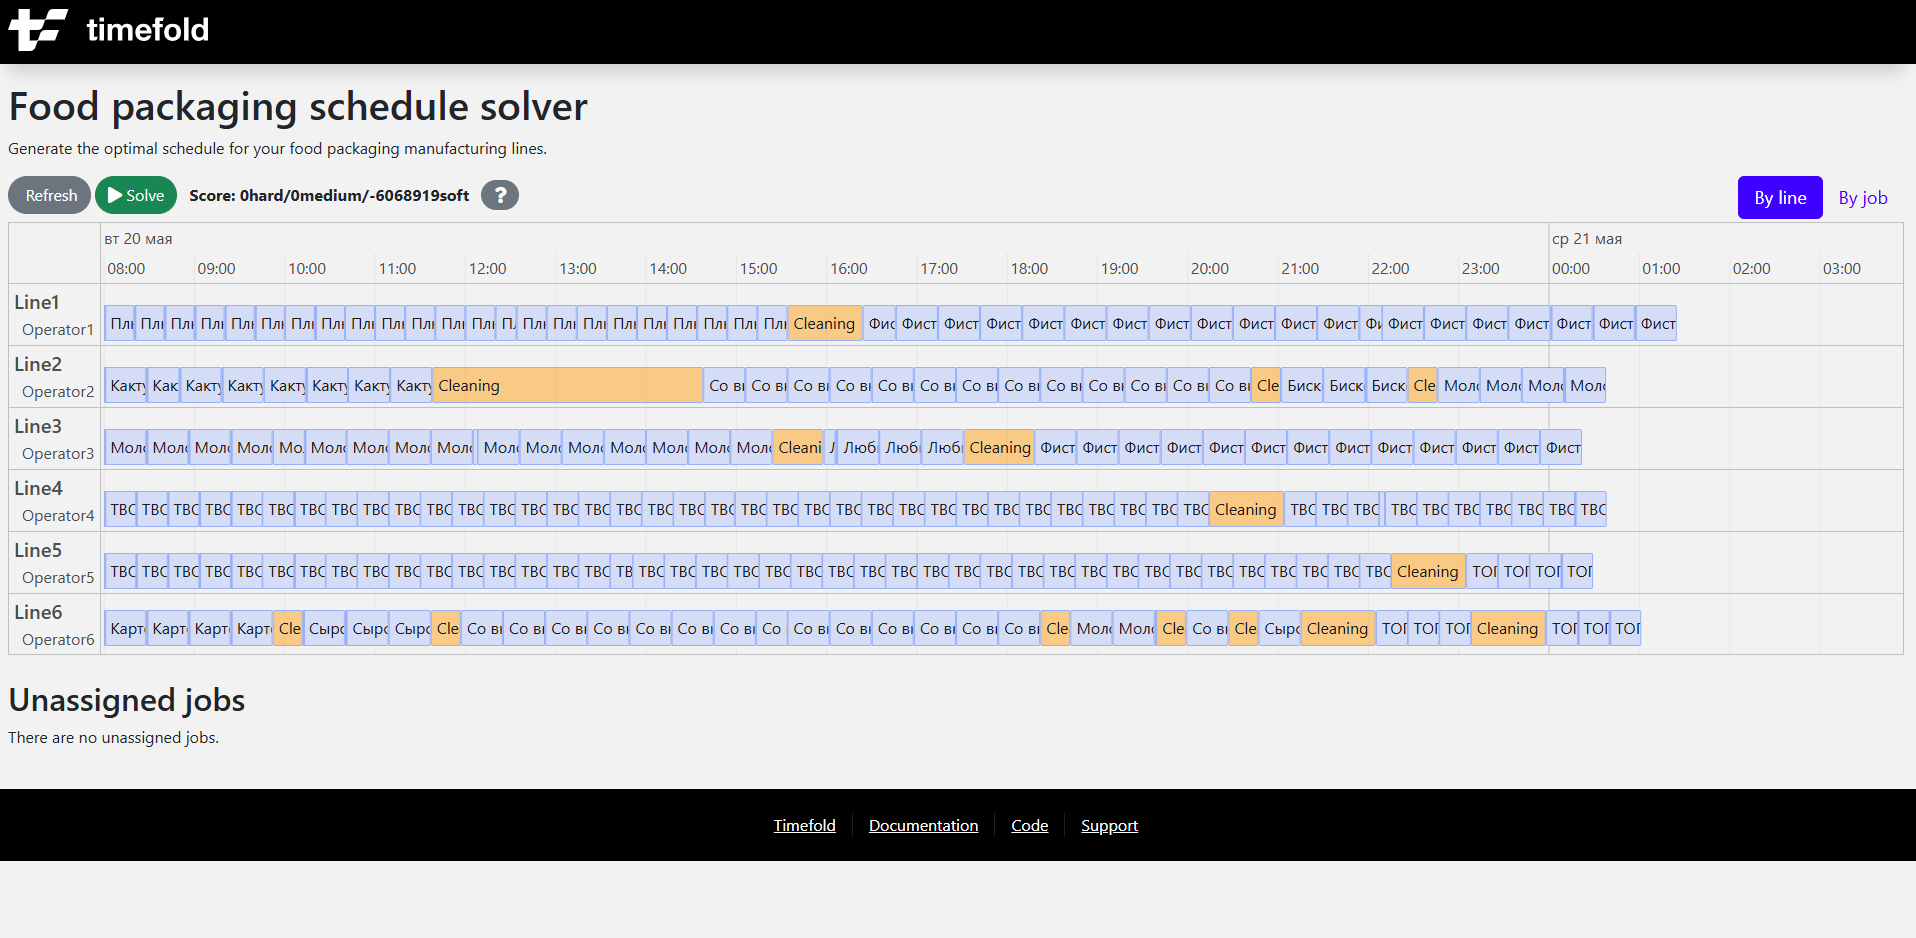
\includegraphics[height = 8 cm, keepaspectratio]{../assets/images/3_1_1Quarkus.png}
		\caption{Визуализация расписания планирования}
		\label{fig:quarkus_3_1}
\end{figure}



\zlabel{lastpagetocount}

\printbibliography

\end{document}
